\section{Full TRM: latent recursion extension}

Full TRM groks on modular addition but does not match Nanda's ${\sim}95\%$ faithful final-logit trig-FVE at 50k steps.
Table~\ref{tab:checkpoint_compare}: final-checkpoint FVE $\HybridFullFVE$; best-FVE mean $\approx 0.30$ (TRM full B).
Ren probes classify most full-TRM seeds as exhibiting Ren fixed-point guessing (Table~\ref{tab:ren_mechanism}).

\paragraph{Checkpoint selection.}
Final checkpoints can show high accuracy with collapsed FVE after cleanup; we analyze grokking- or best-FVE-selected checkpoints for full TRM (Methods, Table~\ref{tab:perseed}).

\paragraph{ACT-depth and HRM probes.}
ACT-depth ablations and reasoning-vs-guessing metrics on $z_H$ show that recursion provides a guess channel before weight circuits stabilize, then partially aligns post-grokking (Appendix~\ref{app:hrm}).

\begin{figure}[h]
  \centering
  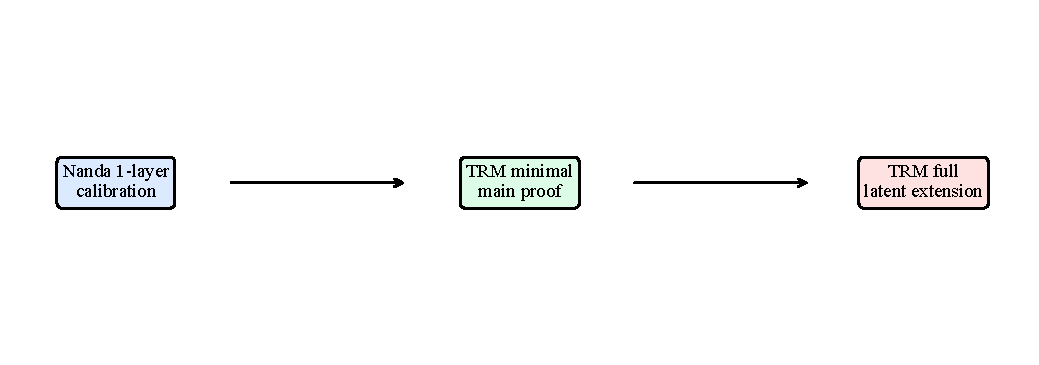
\includegraphics[width=0.95\linewidth]{figures/fig_hybrid_model_ladder.pdf}
  \caption{Hybrid model ladder: Nanda calibration $\to$ TRM minimal (main proof) $\to$ full TRM (extension).}
  \label{fig:ladder}
\end{figure}

\begin{figure}[h]
  \centering
  
\includegraphics[width=0.95\linewidth]{figures/fig_latent_reasoning_modes.pdf}
  \caption{Latent ACT dynamics (full TRM representative seed): mean-field cross-entropy rises and fraction-correct decays across ACT steps, the Ren fixed-point-violation (``guessing'') signature.}
  \label{fig:hrm_modes}
\end{figure}
